\section{Date: 2026-08-10}
\noindent \textbf{Series ID: SUUR0000SAS} 

\noindent This series is titled Chained Consumer Price Index for All Urban Consumers: Services in U.S. City Average and has a frequency of Monthly. The units are Index Dec 1999=100 and the seasonal adjustment is Not Seasonally Adjusted.The observation start date is 1999-12-01 and the observation end date is 2026-06-01.The popularity of this series is 3. \\ 

\noindent \textbf{Series ID: AMBOR1W} 

\noindent This series is titled 1-Week AMERIBOR Term Structure of Interest Rates (DISCONTINUED) and has a frequency of Daily. The units are Percent and the seasonal adjustment is Not Seasonally Adjusted.The observation start date is 2021-06-20 and the observation end date is 2023-12-27.The popularity of this series is 2. \\ 

\subsection{Raw Regression}
\noindent Regresses the two series against each other directly. A significant result here can come just as easily from both series sharing a long-run trend as from any real relationship.

\begin{center}
\begin{tabular}{lclc}
\toprule
\textbf{Dep. Variable:}           & value\_fred\_AMBOR1W & \textbf{  R-squared:         } &     0.930   \\
\textbf{Model:}                   &         OLS          & \textbf{  Adj. R-squared:    } &     0.927   \\
\textbf{Method:}                  &    Least Squares     & \textbf{  F-statistic:       } &     319.1   \\
\textbf{Date:}                    &   Mon, 10 Aug 2026   & \textbf{  Prob (F-statistic):} &  2.29e-15   \\
\textbf{Time:}                    &       12:39:09       & \textbf{  Log-Likelihood:    } &   -23.378   \\
\textbf{No. Observations:}        &            26        & \textbf{  AIC:               } &     50.76   \\
\textbf{Df Residuals:}            &            24        & \textbf{  BIC:               } &     53.27   \\
\textbf{Df Model:}                &             1        & \textbf{                     } &             \\
\textbf{Covariance Type:}         &      nonrobust       & \textbf{                     } &             \\
\bottomrule
\end{tabular}
\begin{tabular}{lcccccc}
                                  & \textbf{coef} & \textbf{std err} & \textbf{t} & \textbf{P$> |$t$|$} & \textbf{[0.025} & \textbf{0.975]}  \\
\midrule
\textbf{const}                    &     -50.4524  &        2.976     &   -16.953  &         0.000        &      -56.595    &      -44.310     \\
\textbf{value\_fred\_SUUR0000SAS} &       0.2849  &        0.016     &    17.863  &         0.000        &        0.252    &        0.318     \\
\bottomrule
\end{tabular}
\begin{tabular}{lclc}
\textbf{Omnibus:}       &  3.117 & \textbf{  Durbin-Watson:     } &    0.261  \\
\textbf{Prob(Omnibus):} &  0.210 & \textbf{  Jarque-Bera (JB):  } &    2.425  \\
\textbf{Skew:}          & -0.614 & \textbf{  Prob(JB):          } &    0.297  \\
\textbf{Kurtosis:}      &  2.147 & \textbf{  Cond. No.          } & 4.58e+03  \\
\bottomrule
\end{tabular}
%\caption{OLS Regression Results}
\end{center}

Notes: \newline
 [1] Standard Errors assume that the covariance matrix of the errors is correctly specified. \newline
 [2] The condition number is large, 4.58e+03. This might indicate that there are \newline
 strong multicollinearity or other numerical problems.

\begin{figure}
\centering
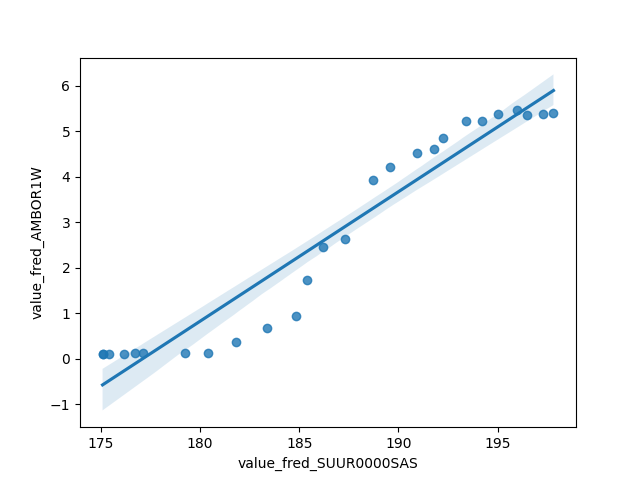
\includegraphics[scale = 0.9]{plots/plot_2026-08-10.png}
\caption{Raw Regression Plot for 2026-08-10}
\end{figure}
\newpage
\subsection{Detrended Regression}
\noindent Regresses the residuals of each series after removing its own linear time trend, so a shared trend can no longer drive the result on its own. A relationship that stays significant here is better evidence of a genuine link between the two series.

\begin{center}
\begin{tabular}{lclc}
\toprule
\textbf{Dep. Variable:}                      & value\_fred\_AMBOR1W\_detrended & \textbf{  R-squared:         } &     0.227   \\
\textbf{Model:}                              &               OLS               & \textbf{  Adj. R-squared:    } &     0.195   \\
\textbf{Method:}                             &          Least Squares          & \textbf{  F-statistic:       } &     7.062   \\
\textbf{Date:}                               &         Mon, 10 Aug 2026        & \textbf{  Prob (F-statistic):} &   0.0138    \\
\textbf{Time:}                               &             12:39:09            & \textbf{  Log-Likelihood:    } &   -23.173   \\
\textbf{No. Observations:}                   &                  26             & \textbf{  AIC:               } &     50.35   \\
\textbf{Df Residuals:}                       &                  24             & \textbf{  BIC:               } &     52.86   \\
\textbf{Df Model:}                           &                   1             & \textbf{                     } &             \\
\textbf{Covariance Type:}                    &            nonrobust            & \textbf{                     } &             \\
\bottomrule
\end{tabular}
\begin{tabular}{lcccccc}
                                             & \textbf{coef} & \textbf{std err} & \textbf{t} & \textbf{P$> |$t$|$} & \textbf{[0.025} & \textbf{0.975]}  \\
\midrule
\textbf{const}                               &   -1.455e-11  &        0.120     & -1.21e-10  &         1.000        &       -0.249    &        0.249     \\
\textbf{value\_fred\_SUUR0000SAS\_detrended} &       0.3703  &        0.139     &     2.657  &         0.014        &        0.083    &        0.658     \\
\bottomrule
\end{tabular}
\begin{tabular}{lclc}
\textbf{Omnibus:}       &  3.443 & \textbf{  Durbin-Watson:     } &    0.285  \\
\textbf{Prob(Omnibus):} &  0.179 & \textbf{  Jarque-Bera (JB):  } &    3.012  \\
\textbf{Skew:}          & -0.790 & \textbf{  Prob(JB):          } &    0.222  \\
\textbf{Kurtosis:}      &  2.467 & \textbf{  Cond. No.          } &     1.16  \\
\bottomrule
\end{tabular}
%\caption{OLS Regression Results}
\end{center}

Notes: \newline
 [1] Standard Errors assume that the covariance matrix of the errors is correctly specified.

\begin{figure}
\centering
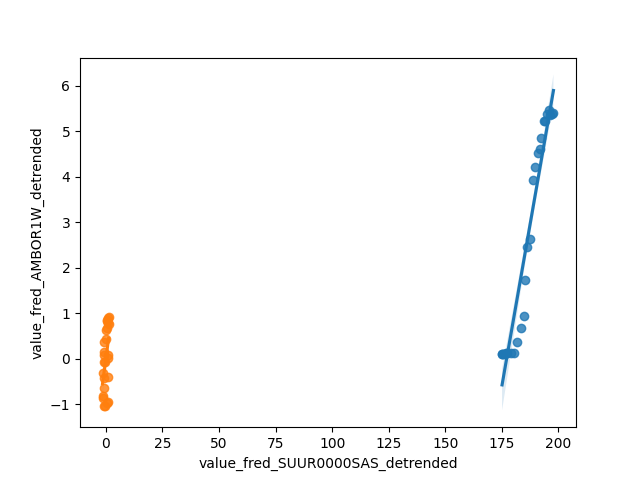
\includegraphics[scale = 0.9]{plots/plot_2026-08-10_detrended.png}
\caption{Detrended Regression Plot for 2026-08-10}
\end{figure}
\newpage
